
\lecture[15]{More on hypothesis testing}{lecture-text}

\subtitle{and checking conditions}

\date{12 March 2015}


\begin{document}

\begin{frame}
  \maketitle
\end{frame}


\begin{frame}{Last time}
  What is, and isn't, implied by ``statistically significant'' (or not).
  \begin{enumerate}
    \item Statistical significance means an observed effect probably wasn't purely the result of chance in sampling,
    \item   \ldots and lack of statistical significance means that it could have been.
    \item The $P$-value says nothing about the size of the effect,
    \item   since the sample size ``acts like a magnifying glass''.
    \item The \alert{effect size} is one way to think about how important an effect is.
    \item Confidence intervals communicate statistical significance,
      as well as information about the absolute size of an effect.
  \end{enumerate}
\end{frame}

\begin{frame}\frametitle<presentation>{Outline}
  \tableofcontents
\end{frame}


\section{Conditions for (best) use of a $t$-test}

\begin{frame}{What are ``conditions''?}

  Statistical tests usually work by finding the probability that 
  \begin{itemize}
    \item something happens,
    \item under a certain generative model.
  \end{itemize}

  \vspace{2em}

  \structure{Example:} The $P$-value for the $t$-test is the probability that 
  \begin{itemize}
    \item the difference in sample means between independent samples from two populations is at least as big as the observed value ($\bar y_1 - \bar y_2$), 
    \item if the two populations have the same mean ($\mu_1 = \mu_2$), and the sampling distribution of the sample mean is Normal.
  \end{itemize}

  \vspace{2em}
  
  \alert{Conditions}, a.k.a.\ ``assumptions'', come from the generative model.
  If they are not true, we might
  \begin{itemize}
    \item have \alert{wrong} $P$-values (misreport the type I error rate)
    \item \structure{and/or} have lower power than a better test \\
      (i.e.\ have more type II errors)
  \end{itemize}

\end{frame}

\subsection{The $t$-test}

%%%%%%
\begin{frame}{the $t$-test}

  \begin{block}{Conditions for the $t$-test}
    \begin{enumerate}
      \item The sampling procedure provides:
        \begin{enumerate}
          \item random, independent samples from large populations,
          \item with the two samples independent of each other.
        \end{enumerate}
      \item The sampling distributions of $\bar Y_1$ and $\bar Y_2$ are
        \begin{enumerate}
          \item close enough to Normal.
      \end{enumerate}
    \end{enumerate}
  \end{block}

  \vspace{2em}

  \structure{Red flags for the $t$-test:}
  \begin{enumerate}
    \item Nonindependence of samples
    \item Small sample sizes 
    \item Skewed distributions
  \end{enumerate}

  \vspace{2em}

  ``Small'' means less than around 20,
  but depends on how close the population distribution is to Normal.

\end{frame}

%%%%%%
\begin{frame}{Simple example}


  \vspace{2em}


  Body weight:
  \begin{center}
    \begin{tabular}{crr}
       & Males & Females \\
       \hline
       $n$ & 2 & 2 \\
       $\bar y$ & 175 & 143 \\
       $s$ & 35 & 34
     \end{tabular}

   \vspace{2em}

   {$t_s=0.93$ and $P=0.45$}\\
   CI for $\bar \mu_1 - \bar \mu_2$: $(-117,181)$
   \end{center}

   \vspace{2em}
  
   \pause
   \alert{The sample sizes are too small} to take the statistics seriously.
   
\end{frame}


%
\begin{frame}{Example: earthquakes}

  % > do.call( cbind, with( subset(quakes,MAG>3), tapply( MAG, weekdays(date), function (x) { list(n=length(x),mean=mean(x),sd=sd(x)) } ) ) )
  %      Friday    Monday    Saturday  Sunday    Thursday  Tuesday   Wednesday
  % n    21        24        31        22        23        24        21       
  % mean 3.33381   3.433333  3.509677  3.309545  3.49913   3.29125   3.382857 
  % sd   0.2215508 0.3715732 0.5015409 0.3381388 0.4162376 0.2501706 0.3910645
  % > with( subset(quakes,MAG>3), t.test( MAG[weekdays(date)=="Sunday"], MAG[weekdays(date)=="Monday"] ) )
  % t = -1.183, df = 43.999, p-value = 0.2432
  % alternative hypothesis: true difference in means is not equal to 0
  % 95 percent confidence interval:
  %  -0.33468020  0.08710444
  %
  % 
  % pdf(file="quakes-mag-hist.pdf",width=3,height=1,pointsize=10)
  % par(mar=c(2,1,0,0)+.1)
  % hist( quakes$MAG[quakes$MAG>3], breaks=25, col=adjustcolor("green",.75), main='', xlab='', ylab='' )
  % dev.off()

  Earthquake magnitudes, for those above magnitude 3.0, on Sundays and Mondays in 2014:
  \begin{center}
    \begin{tabular}{crr}
       & Sundays & Mondays \\
       \hline
       $n$ & 22 & 24 \\
       $\bar y$ & 3.31 & 3.43 \\
       $s$ & 0.34 & 0.37
     \end{tabular}

   \vspace{2em}

   {$t_s=-1.183$ and $P=0.24$}\\
   CI for $\bar \mu_1 - \bar \mu_2$: $(-0.33,0.09)$
   \end{center}

   \pause 
   \begin{center}
     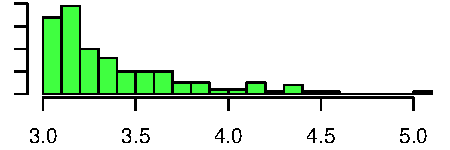
\includegraphics{quakes-mag-hist}
   \end{center}

   \alert{The distribution is skewed,} so with $n\approx 20$, the Normal assumption might not be good.

\end{frame}

%%%%%%%%%%%
\subsection{Transforming the data}

%%%%%%
\begin{frame}{Transformations}

    \begin{block}{Transforming the data}
        means applying a function to the data before doing statistics,\\
        for example
        \[  Y = \text{growth rate} \longrightarrow Y = \log( \text{growth rate} ). \]
    \end{block}

    \vspace{2em}

    \structure{Goal:} make the sampling distribution of $\bar Y$ closer to Normal,\\
    by making the population distribution of $Y$ closer to Normal.

    \vspace{2em}

    \structure{This is a good idea if}
    \begin{enumerate}
        \item The original data do not look Normally distributed,
        \item the transformed data look closer to Normal,
        \item and the statistics you are using require the sampling distribution of $\bar Y$ to be Normal.
    \end{enumerate}

    \vspace{2em}

    \structure{Remember:} informally, ``Normal'' means ``bell-shaped''.

\end{frame}

%
\begin{frame}{Example: earthquakes}

%      do.call( cbind, with( subset(quakes,MAG>3), tapply( log(MAG-3.0), weekdays(date), function (x) { list(n=length(x),mean=mean(x),sd=sd(x)) } ) ) )
%      Friday    Monday    Saturday  Sunday   Thursday  Tuesday   Wednesday
% n    21        24        31        22       23        24        21       
% mean -1.406708 -1.211826 -1.240581 -1.7097  -1.140423 -1.828194 -1.432289
% sd   0.984279  0.9498052 1.234087  1.158273 1.145213  1.35883   1.040219 
%      with( subset(quakes,MAG>3), t.test( log(MAG-3.0)[weekdays(date)=="Sunday"], log(MAG-3.0)[weekdays(date)=="Monday"] ) )
% t = -1.5858, df = 40.736, p-value = 0.1205
% alternative hypothesis: true difference in means is not equal to 0
% 95 percent confidence interval:
%  -1.1320528  0.1363043
% sample estimates:
% mean of x mean of y 
% -1.709700 -1.211826 
%   
%   pdf(file="quakes-log-mag-hist.pdf",width=3,height=1,pointsize=10)
%   par(mar=c(2,1,0,0)+.1)
%   hist( log(quakes$MAG[quakes$MAG>3]-3.0), breaks=25, col=adjustcolor("green",.75), main='', xlab='', ylab='' )
%   dev.off()

Earthquake \alert{$\log(\text{magnitude}-3.0)$}, for those above magnitude 3.0, on Sundays and Mondays in 2014:
  \begin{center}
    \begin{tabular}{crr}
       & Sundays & Mondays \\
       \hline
       $n$ & 22 & 24 \\
       $\bar y$ & -1.71 & -1.21 \\
       $s$ & 1.16 & 0.95
     \end{tabular}

   \vspace{2em}

   {$t_s=-1.60$ and $P=0.12$}\\
   CI for $\bar \mu_1 - \bar \mu_2$: $(-1.13,0.14)$
   \end{center}

   \pause 
   \begin{center}
     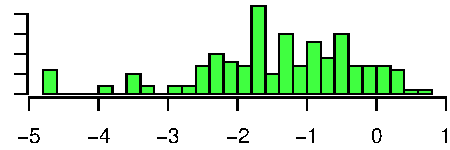
\includegraphics{quakes-log-mag-hist}
   \end{center}

   That looks \emph{closer} to bell-shaped.

\end{frame}


\subsection{Example by simulation}

%%%%%%
\begin{frame}{Real fake data:}
    
  \begin{center}
    (live simulation)
  \end{center}

\end{frame}



%%%%%% %%%%%%
\section{More about hypothesis testing}

\subsection{How to pick the hypotheses?}

%%%%%%
\begin{frame}{Hypotheses}

    Hypothesis testing requires 
    \begin{itemize}
        \item[$H_0$:] null hypothesis
        \item[$H_A$:] alternative hypothesis
    \end{itemize}

    \vspace{2em}

    \structure{Functional difference:} the null hypothesis is what you evaluate the $P$-value with.


\end{frame}


%%%%%%
\begin{frame}{A dialog}
    \begin{itemizew}{1em}
        \item[You:] It looks like $A$s are better than $B$s.  They tend to have more $X$.
        \item[Skeptic:] But what if they're the same, on average, you just happened to see more $X$ in your sample of $A$s?
        \item[You:] Ok, fine.  Suppose, for the sake of argument, that there \alert{isn't} a difference.
            Then let's see what the chance of seeing this much more $X$ is\ldots
    \end{itemizew}

    \vspace{2em}

    \structure{Note:}
    Often (like in this example), 
        \[ H_0: \mu_1 = \mu_2 , \]
    but not always.

\end{frame}


%%%%%%
\begin{frame}{What are the hypotheses?}

  To study the effect of latitude on body size in urban mammals, 
  we took two samples of mice, from Seattle and Los Angeles,
  and compared their mean body mass.

    \vspace{2em}
    \pause

  The El Ni\~no--Southern Oscillation (ENSO) effect produces increased rainfall along the entire Pacific coast about every four years.
  We collect rainfall data from many ENSO years, and compare the Seattle--Los Angeles difference to the usual level,
  knowing that Seattle gets on average 23 inches of rain per year more than Los Angeles.


    \vspace{2em}
    \pause

  We have genetic data from a genetic variant in 1,000 healthy people and 1,000 people with a disease,
  and would like to find out whether the genetic variant affects the chances of getting the disease.

\end{frame}



\subsection{Interpreting $P$-values}


%%%%%%
\begin{frame}{$P$-values}

    \begin{block}{}
      The \alert<1>{$P$-value} of a \alert<2>{result} is the probability of seeing a result \alert<3>{so extreme}, \alert<4>{if $H_0$ is true}.
    \end{block}

    \vspace{2em}
          \pause

    \begin{itemizew}{4em}
        \item[``result'':] the test statistic (ex: $\bar y_1 - \bar y_2$)
          \pause
        \item[``so extreme'':] defined by $H_A$ (ex: $\bar y_1 - \bar y_2 > C$)
          \pause
        \item[``if $H_0$ is true'':] how to compute the probability.
    \end{itemizew}

\end{frame}


\subsection{Medical testing example}

%%%%%%
\begin{frame}{Example:}

    A medical test for an illness:
    \begin{itemize}
        \item 1\% of population has the illness,
        \item 80\% chance of (true) detection if patient has the illness, 
        \item 5\% chance of (false) detection if patient does not.
    \end{itemize}

    \vspace{2em}

    With $H_0$: patient is healthy,
    if we test 1,000 patients, how many do we expect of:
    \begin{enumerate}
        \item falsely rejected null hypotheses? (type I errors)
        \item falsely accepted null hypotheses? (type II errors)
    \end{enumerate}

    \vspace{2em}
    \pause

    If you get a positive result,
    what's the chance that you have the illness?

    \vspace{2em}
    \pause

    \structure{True or false:} 
    We have found significant evidence for $H_A$ with $P<5\%$,
    so the probability that $H_0$ is true is 5\%.

    \vspace{2em}
    \pause

    What is a true statement similar to the above?


\end{frame}




\section<article>{Summary}
\section<presentation>*{Summary}

\begin{frame}{Summary}
  \begin{enumerate}
  \item The null hypothesis determines the conditions you use to calculate the $P$-value.
  \item If the conditions do not hold, the $P$-value may be wrong,
  \item or you might just be better off using a different test.
  \item The $t$-test depends on the sampling distribution of the sample mean being Normal;
  \item for this purpose, the closer the data are to Normal the better;
  \item sometimes, transforming the data helps.
  \end{enumerate}
\end{frame}

% homework
\begin{frame}{Homework}
  \begin{center}

  7.8.2

  \vspace{2em}

  7.9.1


  \end{center}
\end{frame}


\end{document}





